
\section{Transformer and Attention}

The Transformer is a mechanism that is based entirely on attention. Strictly speaking this is not the attention explored in the Sequence to Sequence model in Chapter 1, though there are some similarities. It is a model that uses no recurrent components and no convolution components. 

Recurrent components have some negative qualities. Recurrent components are hard to run with batch input data. Also they do not work with very long data strings. 

If a batch of data is to be cycled through a recurrent component, all that data has to go through the component at the first cardinal position before it is cycled through the second or third position. In the first time step everything needs to go through the first RNN module. Then the data can be moved along to the second RNN  module in the second time step.

Also because the RNN is so heavy with Neural Network components, many weights and biases, though they can remember patterns, they loose some information with every pass. This is why there is a practical limit to the length of the input sequences that the typical RNN can use. This is why the length of sentences in network models that use the RNN are short.

Transformers use no RNN components. Their operations can be parallelized so that large batches of data can be processed at once during the same time step. 

Longer sequences can be considered as well, so Transformer input can contain longer english language sentences and even paragraphs.

%\subsection*{Model Overview}
Attention mechanisms are used in a similar way in three places in the model. The first implementation of the Self Attention is discussed below.

It should be noted that input to the Transformer is strings of words from a desired input language. Output is similarly words in a given language. Input words are treated very much the way that they are in Sequence to Sequence models. A word is translated to a number and that number indexes an entry in a word-to-vector table. From that time forward a word is represented by a vector of floating point numbers. In a transformer this word vector can be large. In the original paper Vaswani et al (2017)\cite{Vaswani2017AttentionIA} use a vector size of 512. 

\subsection*{Scaled Dot-Product Attention}

The Transformer has a signature self-attention mechanism. This is possibly one third of the entire Transformer mechanism, but a variety shows up in the other two-thirds. 

The first thing that happens is the input word is converted to three other values. These new vectors are like the input vector but they have a smaller dimensionality. Converting the word vector in this way is accomplished by three simple matrix multiplication operations.

In the diagram below a simple conversion of this type is illustrated. In the diagram we convert a vector with dimension of 1x3 to a dimension of 1x2. In reality we are converting a vector from 1x512 to 1x64. This is a division of 8.



\begin{figure}[H]
	\begin{center}
		
	
	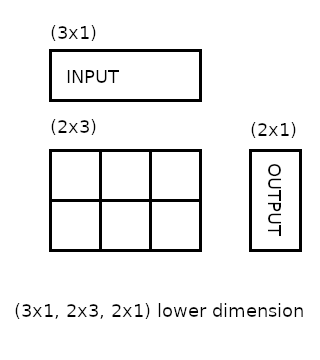
\includegraphics[scale=0.5]{diagram-mat01}
\end{center}
	\caption[Lowering Dimensionality]{Lowering Dimensionality}
	
	%\addcontentsline{lof}{section}{Loss and Accuracy}
\end{figure}


One thing we want to do is to preserve the dimension of our vector. We start with a 512 sized floating point vector and after some processing we want to return to the same size. Before that is done the vector is processed at the smaller size of 64. 

In this self-attention scheme three vectors are actually required. All three vectors are sized 64, and all three are converted by separate matrix multiplication operations. The weights to convert each of the three vectors are different. For this reason the new smaller vectors are all different.

The smaller vectors individually are called q,k, and v. They can also be referred to as larger matrices. The new vector matrices are denoted as Q, K, and V. Q stands for Query. K stands for Key. V stands for Value. 

The Query value is multiplied by the Key values from all vectors in the input. This multiplication is 'dot-product' multiplication. When it is done all keys will have low output except those that are closest to the Query. Then the results are passed through a softmax function. When this is complete there will be a single vector that is close to 1 and another group of vectors that are all close to 0.

The vector produced by multiplying the softmax with the V values of every word produces a single word vector that is close to its original value, and many others that are near zero.

This formula from Vaswani et al (2017)\cite{Vaswani2017AttentionIA} 
shows the process.

$$
Attention(Q,K,V)=softmax(\dfrac{QK^T}{\sqrt{d_k}})V
$$

Here the value of $\sqrt{d_k}$ is used to limit the size of the $QK^T$ output. Without this the softmax function has to deal with much larger numbers. Smaller numbers for the softmax are preferred. 

The function can actually perform this on large matrices with high dimensionality, in parallel. This parallel matrix operation increases the speed of training.

In the green triangle in the Figure 2.2 we preform the multiplication and selection that was just described.

\begin{figure}[H]
	\begin{center}
		
		
		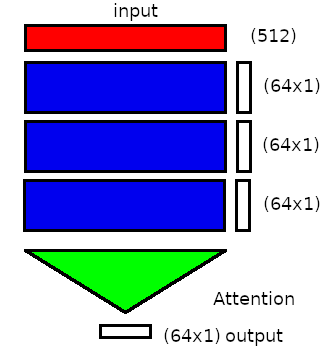
\includegraphics[scale=0.5]{diagram-mat03-64}
	\end{center}
	\caption[Attention Output]{Attention Output}
	
	%\addcontentsline{lof}{section}{Loss and Accuracy}
\end{figure}




Finally the output we calculated above must be returned somehow to the input dimensionality. This is accomplished by duplicating the procedure described eight times with eight separate weights. When this is done the output of the attention mechanism is concatinated together, returning the output to the proper size.

This multi-headed approach allows different heads to learn different types of relationships, and then when they are summed together the learned relations are recovered and contribute to the output.

\begin{figure}[H]
	\begin{center}
		
	
	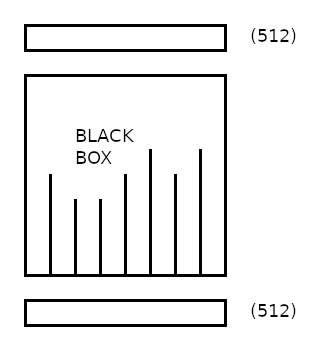
\includegraphics[scale=0.5]{diagram-mat02}
\end{center}
	\caption[Matching Input and Output]{Matching Input and Output}
	
	%\addcontentsline{lof}{section}{Loss and Accuracy}
\end{figure}


Later the output is passed through a feed forward network. After that it is combined with the original input again through addition. Then the vectors are normalized. This makes sure that the values are all within reasonable ranges.

This describes the encoder section. There are two other attention segments. Together these two sections combine to form the decoder section.

\subsection*{Transformer - General}
While the encoder takes in the entire input and attends to whatever portion of that input it finds to be important, the decoder is interested in producing one token at a time. 

During inference it produces a token and then it adds to that token, one at a time, until the decoding is finished. It can attend to any part of the output it has already produced. During training the decoder is exposed to the target sequence under a mask. The mask prohibits the decoder from seeing parts of the target that it should not. This mimics the inference setup and still allows for large input matrices.

\begin{figure}[H]
	\begin{center}
		
		
		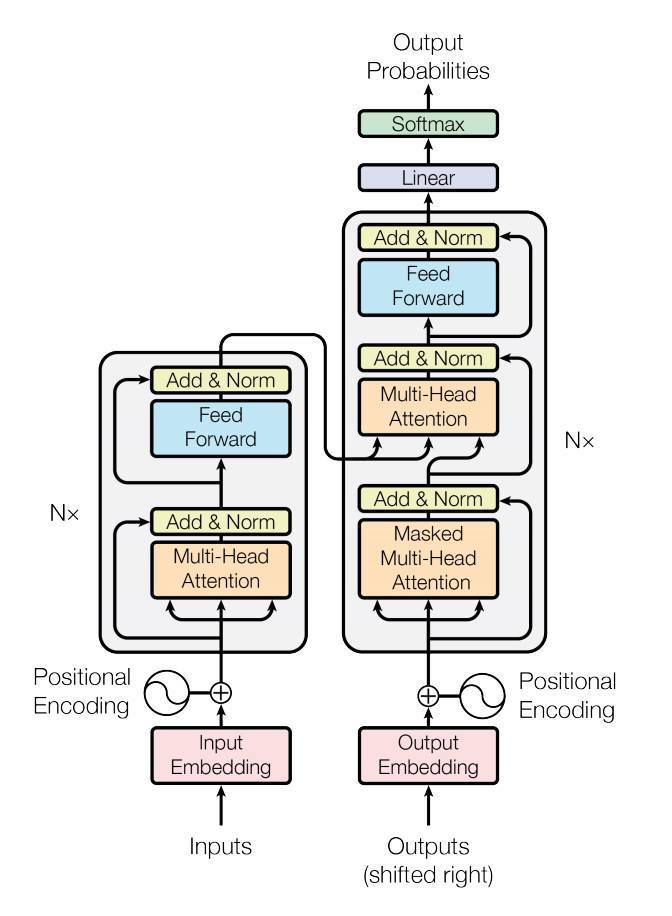
\includegraphics[scale=2.0]{diagram-mat04}
	\end{center}
	\caption[Transformer Encoder and Decoder]{Transformer Encoder and Decoder - Vaswani et al(2017)\cite{Vaswani2017AttentionIA}}
	
	%\addcontentsline{lof}{section}{Loss and Accuracy}
\end{figure}

The Transformer model takes large memory resources, large corpus resources, and large training time resources. Without these components the Transformer is not usable for many projects.